\chapter{Result and Discussion}
\notocsection{Evaluation Metrics Overview}
To assess the performance of the Super-Resolution Generative Adversarial Network (SRGAN) model, both quantitative and qualitative metrics were utilized:

\textbf{Quantitative Metrics}
\begin{itemize}
    \item PSNR (Peak Signal-to-Noise Ratio): Measures the fidelity of the reconstructed image compared to the high-resolution (HR) image. 
    \item SSIM (Structural Similarity Index Measure): Evaluates image quality based on luminance, contrast, and structure similarity.
\end{itemize}
\begin{figure}[h!]
    \centering
    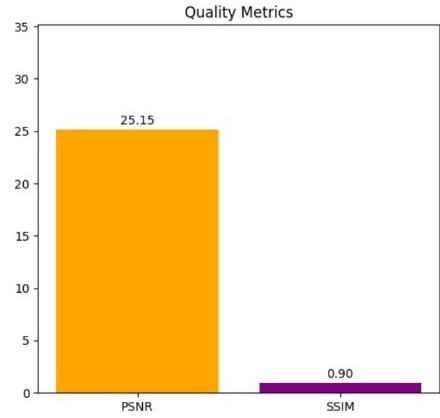
\includegraphics[width=0.6\textwidth]{image/gan.jpg} % <-- Update with your actual file path
    \caption{PSNR AND SSIM}
    \label{fig:workflow}
\end{figure}

\begin{table}[h]
\centering
\renewcommand{\arraystretch}{1.5}
\begin{tabular}{|c|c|p{8cm}|}
\hline
\textbf{PSNR (dB) Range} & \textbf{Quality} & \textbf{Description} \\
\hline
More Than 40 & Excellent & Indistinguishable from the original \\
\hline
30 -- 40 & Good & Very slight differences, barely noticeable \\
\hline
25 -- 30 & Fair / Acceptable & Noticeable noise or blur, but still usable \\
\hline
20 -- 25 & Poor & Degraded quality, visible artifacts \\
\hline
Less Than 20 & Bad & Very poor quality, heavy distortion \\
\hline
\end{tabular}
\caption{PSNR Quality Assessment range}
\end{table}

\vspace{0.5cm}
\begin{table}[h]
\centering
\renewcommand{\arraystretch}{1.5}
\begin{tabular}{|c|c|p{8cm}|}
\hline
\textbf{SSIM Value Range} & \textbf{Quality} & \textbf{Description} \\
\hline
0.95 -- 1.00 & Excellent & Structure and details very well preserved \\
\hline
0.90 -- 0.95 & Very Good & Small differences, high visual similarity \\
\hline
0.80 -- 0.90 & Good & Moderate quality, slight structural differences \\
\hline
0.60 -- 0.80 & Fair & Noticeable structural loss, acceptable in some cases \\
\hline
Less Than 0.60 & Poor & Strong structural degradation, visually different \\
\hline
\end{tabular}
\caption{SSIM Quality Assessment range}
\end{table}


% Precision, Recall, and F1 Score: For classification-based tasks such as image enhancement assessment or evaluation using a classifier.

\textbf{Image Quality Results}

From the image which compares the Original Image, the Enhanced Image, and the Quality Metrics, we extract the following:

\begin{enumerate}
    \item \textbf{PSNR: 25.15 dB}\\
    This indicates a decent level of reconstruction fidelity. Values above 25 dB are generally considered acceptable for image super-resolution, with 30+ being ideal for very high-quality reconstruction.
    
    \item \textbf{SSIM: 0.90}\\
    A high SSIM (close to 1.0) shows that the enhanced image is structurally very similar to the original HR image, indicating excellent quality preservation in terms of shapes, textures, and structural details.
\end{enumerate}

\begin{figure}[h!]
    \centering
    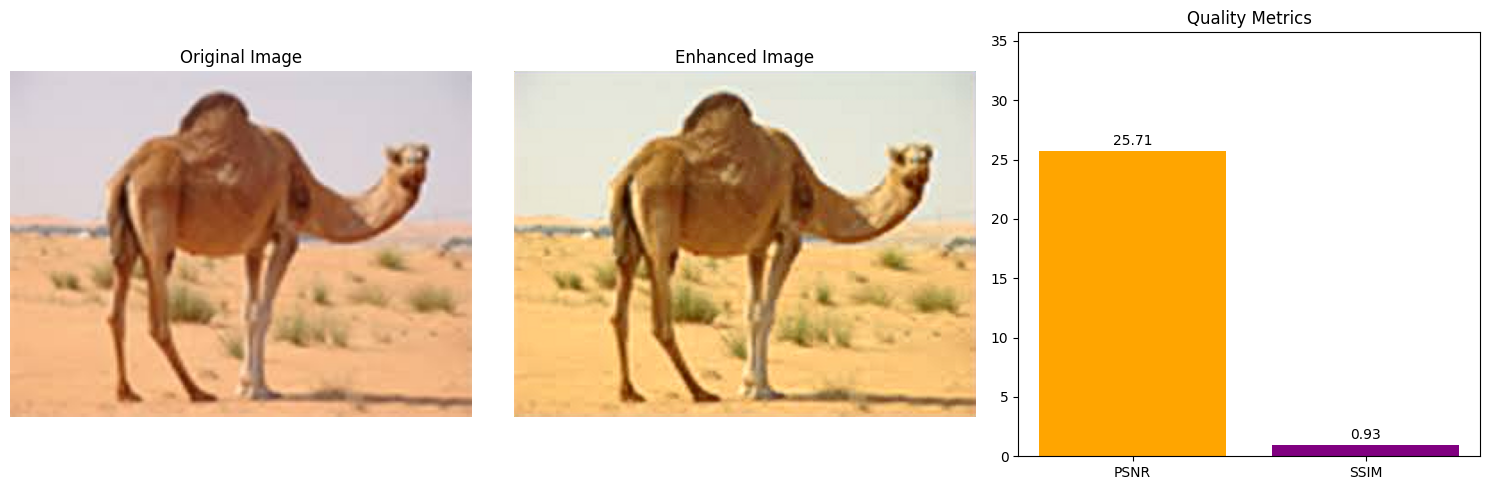
\includegraphics[width=1\textwidth]{image/ESRGAN output 4.png} % <-- Update with your actual file path
    \caption{ESRGAN Result }
    \label{fig:workflow}
\end{figure}


\notocsection{Classification-Based Evaluation}
This image provides a confusion matrix and classification metrics for some binary evaluation (likely distinguishing between high-quality vs. low-quality or real vs. generated):

\begin{table}[h]
\centering
\renewcommand{\arraystretch}{1.5}
\begin{tabularx}{0.8\textwidth} { 
  | >{\raggedright\arraybackslash}X 
  | >{\centering\arraybackslash}X 
  | >{\raggedleft\arraybackslash}X | }\hline
% \resizebox{0.9\textwidth}{!}{ % Adjust 0.9 to make it smaller or larger
\textbf{Metric} & \textbf{Value} \\
\hline
Precision & 0.8018 \vspace{0.4cm} \\
\hline

Recall    & 0.9563 \vspace{0.4cm}\\
\hline

F1 Score  & 0.8723 \vspace{0.4cm} \\
\hline
\end{tabularx}
\caption{Evaluation Metrics}
\label{tab:evaluation_metrics}
\end{table}

% \begin{figure}[h!]
%     \centering
%     
\includegraphics[width=0.93\textwidth]{image/1f1.jpg} % <-- Update with your actual file path
%     \caption{Evaluation Matrics}
%     \label{fig:workflow}
% \end{figure}
\begin{enumerate}
    \item \textbf{Precision: 0.8018}\\
    Indicates that 80.18\% of the predicted positive cases were correct.
    
    \item \textbf{Recall: 0.9563}\\
    Very high recall implies that the model was able to correctly identify most of the actual positive cases.
     
    \item \textbf{F1 Score: 0.8723}\\
    The harmonic mean of precision and recall. A high F1 score indicates a balanced and effective classification performance.
\end{enumerate}
\begin{figure}[h!]
    \centering
    \fbox{%
        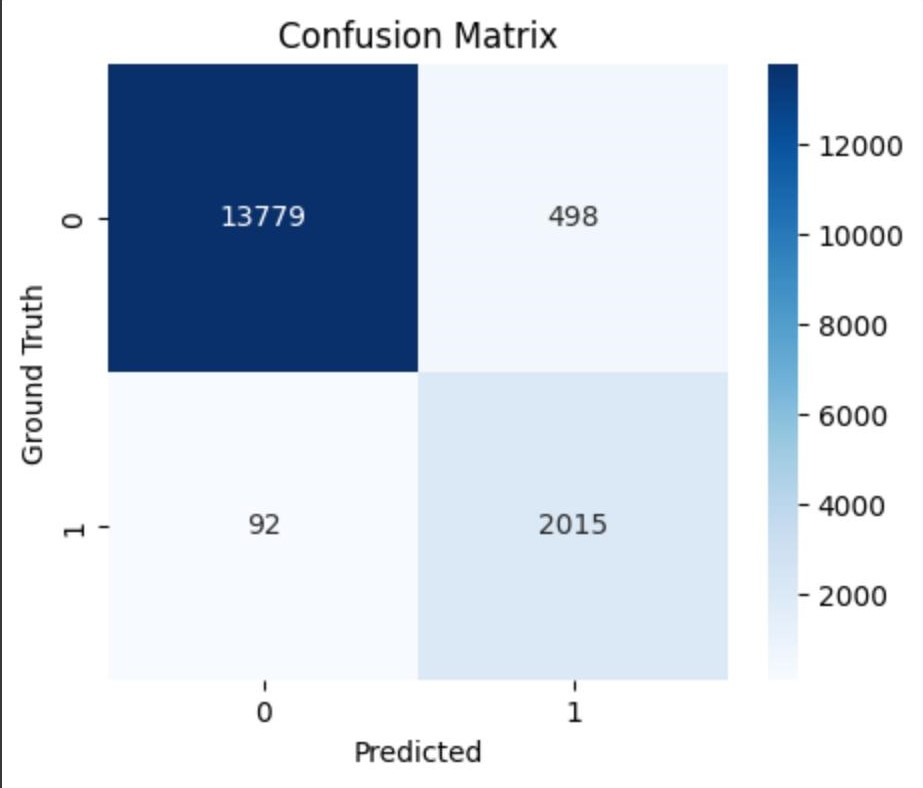
\includegraphics[width=0.6\textwidth]{image/cm.jpg} % <-- Update with your actual file path
    }
    \caption{Confusion matrix}
    \label{fig:workflow}
\end{figure}

\notocsection{Comparative Analysis: CNN vs SRGAN}
To evaluate the effectiveness of different super-resolution approaches, we compare the performance of a traditional CNN-based enhancement model and the SRGAN (Super-Resolution Generative Adversarial Network).

The comparison is based on:

\begin{itemize}
    \item Visual (Qualitative) quality
    
    \item Quantitative metrics: PSNR and SSIM
\end{itemize}

\begin{table}[h!]
    \centering
    \caption{Comparison of CNN and SRGAN Models on Image Quality Metrics}
    \resizebox{0.9\textwidth}{!}{ % Adjust 0.9 to make it smaller or larger
    \begin{tabularx}{\textwidth}{|>{\centering\arraybackslash}m{3cm}|>{\centering\arraybackslash}m{2.5cm}|>{\centering\arraybackslash}m{2.5cm}|X|}
        \hline
        \textbf{Metric} & \textbf{CNN Model} & \textbf{SRGAN Model} & \textbf{Interpretation} \\
        \hline
        PSNR (dB) & 7.09 & 25.15 & SRGAN has a significantly higher PSNR, indicating far less distortion and better image reconstruction. \\
        \hline
        SSIM & 0.18 & 0.90 & SRGAN's structural similarity to the original image is much higher, showing it retains textures and details far better. \\
        \hline
    \end{tabularx}
    }
\end{table}

% \begin{table}[h]
% \centering
% \caption{Evaluation Metrics}
%  \resizebox{0.6\textwidth}{!}{ % Adjust 0.9 to make it smaller or larger

% \begin{tabularx}{\textwidth}{|>{\centering\arraybackslash}m{3cm}|>{\centering\arraybackslash}m{2.5cm}|>{\centering\arraybackslash}m{2.5cm}|X|}\hline
% % \resizebox{0.9\textwidth}{!}{ % Adjust 0.9 to make it smaller or larger
% \textbf{Metric} & \textbf{Value} \\
% \hline
% Precision & 0.8018 \\
% Recall    & 0.9563 \\
% F1 Score  & 0.8723 \\
% \hline
% \end{tabularx}
% }
% % \label{tab:evaluation_metrics}
% \end{table}




In terms of quantitative performance, the SRGAN model significantly outperforms the CNN-based enhancement model. The Peak Signal-to-Noise Ratio (PSNR) of the CNN model is recorded at just 7.09 dB, indicating a high level of distortion in the reconstructed image. In contrast, the SRGAN model achieves a PSNR of 25.15 dB, reflecting much better reconstruction quality with reduced noise and artifacts. Similarly, the Structural Similarity Index (SSIM), which measures the perceptual similarity between the original and enhanced images, is only 0.18 for the CNN output, suggesting a poor structural match. The SRGAN output, however, attains an SSIM of 0.90, demonstrating excellent preservation of structural details and textures. 
% These metrics clearly indicate that SRGAN is more effective in producing high-quality, perceptually faithful images compared to the CNN-based approach.




\begin{figure}[h!]
    \centering
    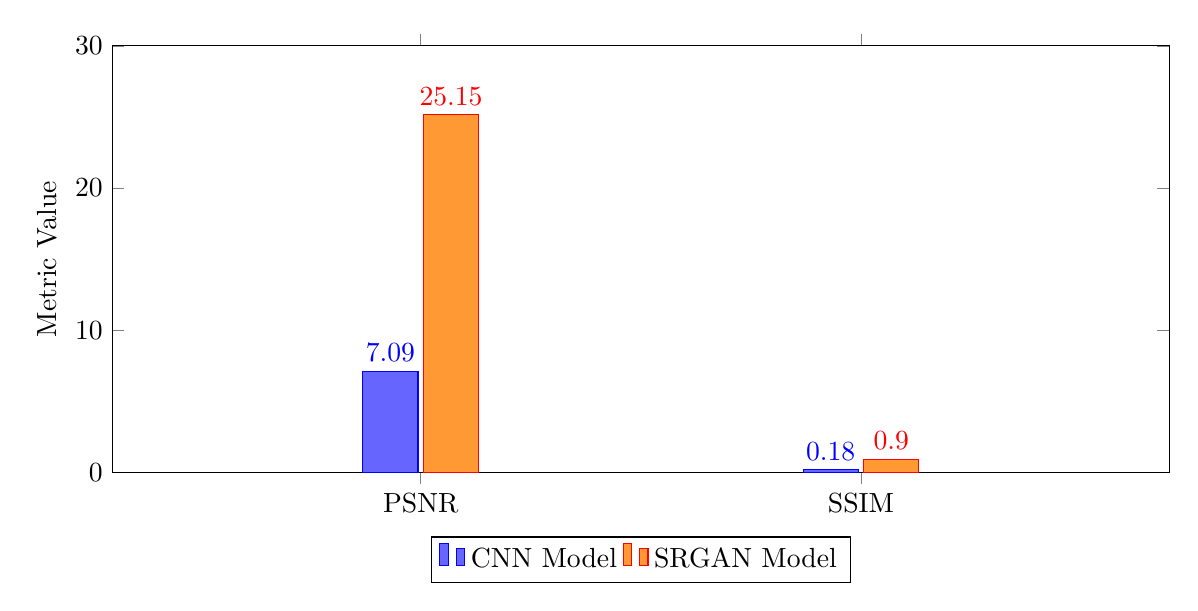
\begin{tikzpicture}
        \begin{axis}[
            ybar,
            bar width=.7cm,
            width=15cm,
            height=7cm,
            enlarge x limits=0.7,
            legend style={at={(0.5,-0.15)},
                anchor=north,legend columns=-1},
            ylabel={Metric Value},
            symbolic x coords={PSNR, SSIM},
            xtick=data,
            nodes near coords,
            nodes near coords align={vertical},
            ymin=0,
            ymax=30
        ]
        \addplot+[style={fill=blue!60}] coordinates {(PSNR,7.09) (SSIM,0.18)};
        \addplot+[style={fill=orange!80}] coordinates {(PSNR,25.15) (SSIM,0.90)};
        \legend{CNN Model, SRGAN Model}
        \end{axis}
    \end{tikzpicture}
    \caption{Comparison of CNN and SRGAN Models on PSNR and SSIM}
    \label{fig:cnn_vs_srgan_chart}
\end{figure}


\notocsection{Qualitative (Visual) Comparison}
\textbf{CNN-Enhanced Image}
\begin{itemize}
    \item Appears dark, heavily distorted, and visually degraded.
    
    \item Critical features such as facial details, hands, and food items are poorly reconstructed.
    
    \item Overall perceptual quality is very low, making the image almost unrecognizable.
\end{itemize}

\textbf{SRGAN-Enhanced Image }
\begin{itemize}
    \item Retains fine details such as facial lines, hand shape, and hair texture.
     
    \item The color distribution and contrast are more natural.
    
    \item Very close in appearance to the original image, showing excellent visual fidelity.
\end{itemize}

\vspace{0.7cm}

\begin{figure}[h]
    \centering
    
\includegraphics[width=0.3\textwidth]{image/org.jpg}
    \hfill
    
\includegraphics[width=0.3\textwidth]{image/gan1.jpg}
    \hfill
    
\includegraphics[width=0.3\textwidth]{image/cnn.jpg}
    \caption{a) Original image b) SRGAN-Enhanced Image c) CNN Enhanced Image}
    \label{fig:three_image}
\end{figure}
\begin{figure}[h!]
    \centering
    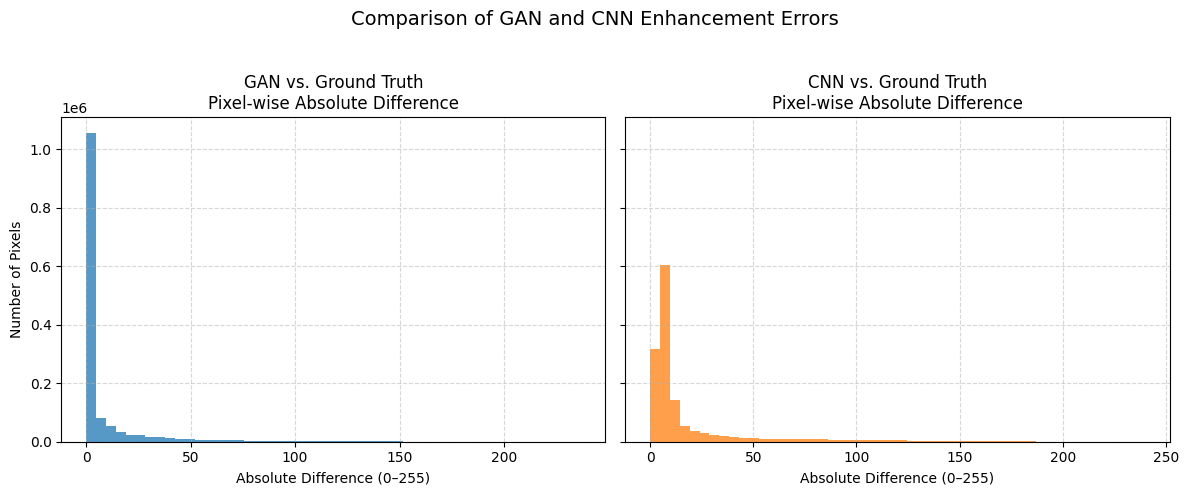
\includegraphics[width=1\textwidth]{image/download.png} % <-- Update with your actual file path
    \caption{Pixel-wise absolute difference}
    \label{fig:workflow}
\end{figure}
\textbf{Interpretation}
\begin{itemize}
    \item Histogram peak near 0 indicates many pixels match the ground truth closely.
    
    \item A narrower GAN histogram (taller near 0, shorter tails) means GAN produces fewer large errors.

    \item A wider CNN histogram (more mass at higher differences) shows CNN struggles to match fine details.
    \end{itemize}
    Visually, SRGAN produces an image nearly identical to the original, whereas the CNN model fails to reconstruct important image details.






% \begin{figure}[h!]
%     \centering
%     \begin{subfigure}[b]{0.45\textwidth}
%         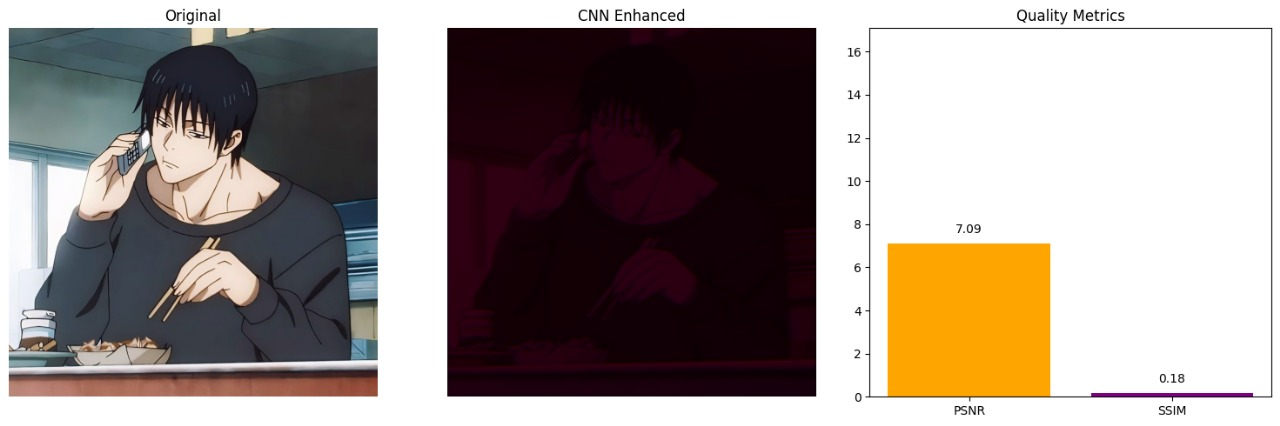
\includegraphics[width=\textwidth]{image/cnn1.jpg}
%         \caption{First Image}
%         \label{fig:image1}
%     \end{subfigure}
%     \hspace{1cm} % Adjust space between images
%     \begin{subfigure}[b]{0.45\textwidth}
%         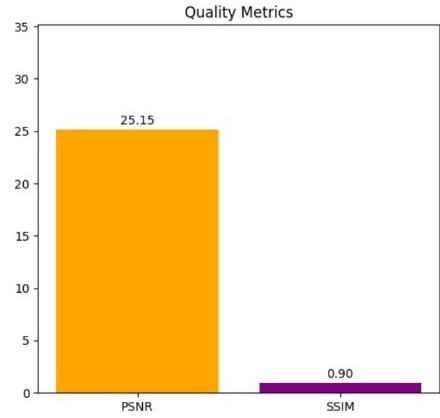
\includegraphics[width=\textwidth]{image/gan.jpg}
%         \caption{Second Image}
%         \label{fig:image2}
%     \end{subfigure}
%     \caption{Comparison of two images}
%     \label{fig:side_by_side}
% \end{figure}





















% \begin{figure}[htbp]
%     \centering
%     \begin{subfigure}[b]{0.22\textwidth}
%         \includegraphics[width=\textwidth]{r1.jpg}
%         \caption{Result 1}
%     \end{subfigure}
%     \begin{subfigure}[b]{0.22\textwidth}
%         \includegraphics[width=\textwidth]{r2.jpg}
%         \caption{Result 2}
%     \end{subfigure}
%     \begin{subfigure}[b]{0.22\textwidth}
%         \includegraphics[width=\textwidth]{r3.jpg}
%         \caption{Result 3}
%     \end{subfigure}
%     \begin{subfigure}[b]{0.22\textwidth}
%         \includegraphics[width=\textwidth]{r4.jpg}
%         \caption{Result 4}
%     \end{subfigure}
    
%     \vspace{0.5cm}
    
%     \begin{subfigure}[b]{0.22\textwidth}
%         \includegraphics[width=\textwidth]{r5.jpg}
%         \caption{Result 5}
%     \end{subfigure}
%     \begin{subfigure}[b]{0.22\textwidth}
%         \includegraphics[width=\textwidth]{r6.jpg}
%         \caption{Result 6}
%     \end{subfigure}
%     \begin{subfigure}[b]{0.22\textwidth}
%         \includegraphics[width=\textwidth]{r7.jpg}
%         \caption{Result 7}
%     \end{subfigure}
%     \begin{subfigure}[b]{0.22\textwidth}
%         \includegraphics[width=\textwidth]{r8.jpg}
%         \caption{Result 8}
%     \end{subfigure}
    
%     \caption{Super-resolution results generated by the proposed GAN model.}
%     \label{fig:results}
% \end{figure}


